\chapter{Results}


\section{Simulation}
\begin{figure}[htb]
	\begin{center}
		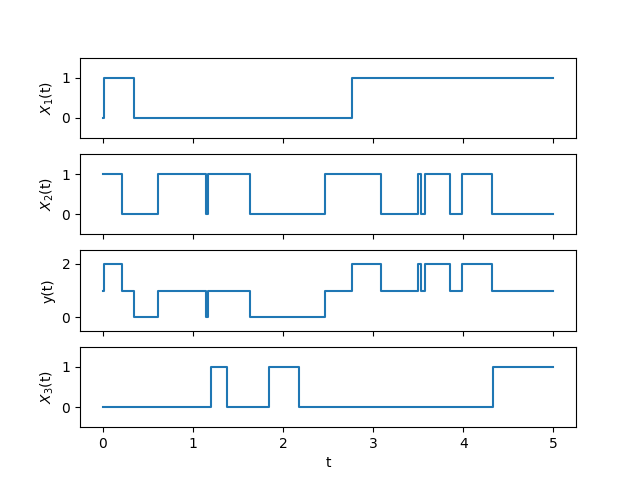
\includegraphics[width=.50\textwidth]{figures/traj}
		\caption{Sampled trajectories}
		\label{fig:traj}
	\end{center}
\end{figure}
\begin{figure}[htb]
	\begin{center}
		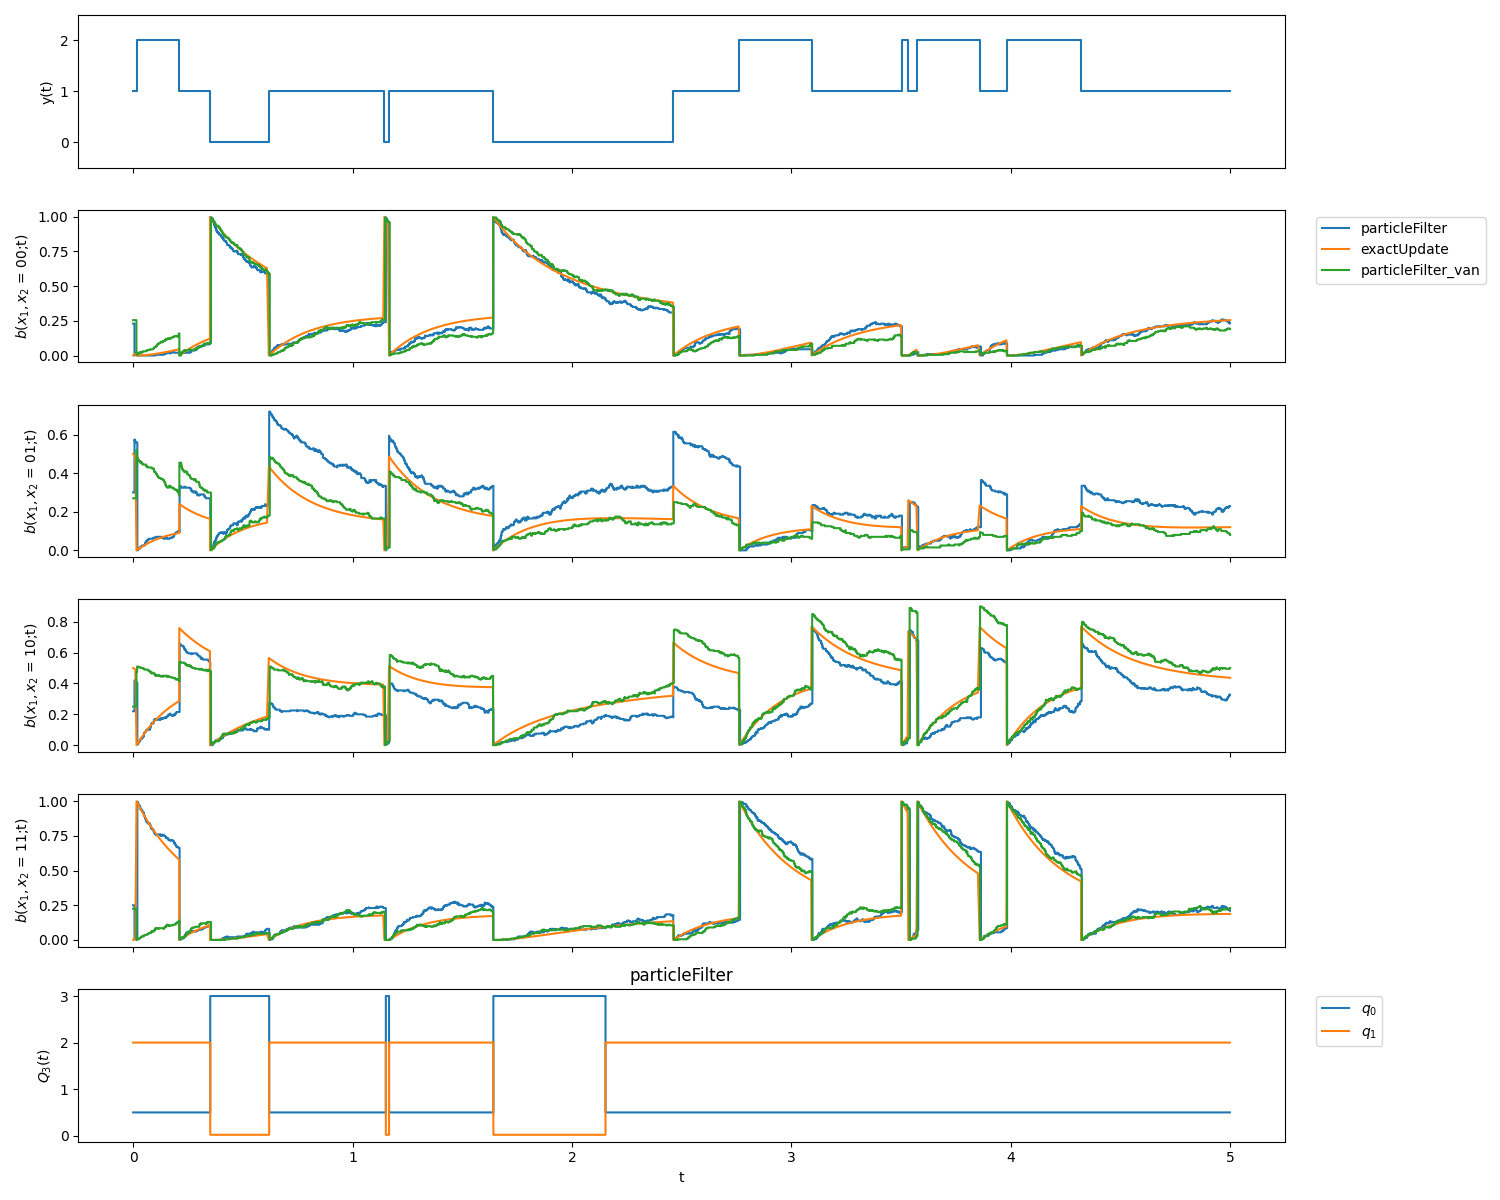
\includegraphics[width=.50\textwidth]{figures/b_q_traj}
		\caption{Belief state and $ Q_3 $ trajectories}
		\label{fig:b_q_traj}
	\end{center}
\end{figure}

\section{Results}
\subsection{Maximum Likelihood Estimation}
$\psi_{true} =
\begin{bmatrix} \vspace{-2pt}
	1 & 0 & 0 \\  \vspace{-2pt}
	0 & 1 & 0 \\  \vspace{-2pt}
	0 & 1 & 0 \\  \vspace{-1pt}
	0 & 0 & 1
\end{bmatrix}$
$\psi_{0} =
\begin{bmatrix} \vspace{-2pt}
1 & 0 & 0 \\  \vspace{-2pt}
0 & 1 & 0 \\  \vspace{-2pt}
0 & 1 & 0 \\  \vspace{-1pt}
0 & 0 & 1
\end{bmatrix}, 
\psi_{1} =
\begin{bmatrix} \vspace{-2pt}
0 & 0 & 1 \\  \vspace{-2pt}
0 & 1 & 0 \\  \vspace{-2pt}
1 & 0 & 0 \\  \vspace{-1pt}
0 & 0 & 1 
\end{bmatrix},
\psi_{2} =
\begin{bmatrix} \vspace{-2pt}
0 & 0 & 1 \\  \vspace{-2pt}
1 & 0 & 0 \\  \vspace{-2pt}
0 & 0 & 1 \\  \vspace{-1pt}
0 & 1 & 0  
\end{bmatrix}$
\begin{figure}[htb]
	\begin{subfigure}{.5\textwidth}
		\centering
		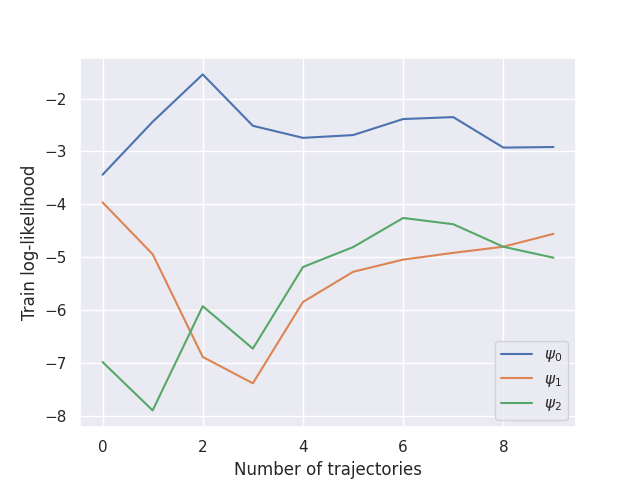
\includegraphics[width=1\linewidth]{figures/llh_[1.0, 0.0, 0.0]}
		\caption{}
		\label{fig:sfig1}
	\end{subfigure}%
	\begin{subfigure}{.5\textwidth}
		\centering
		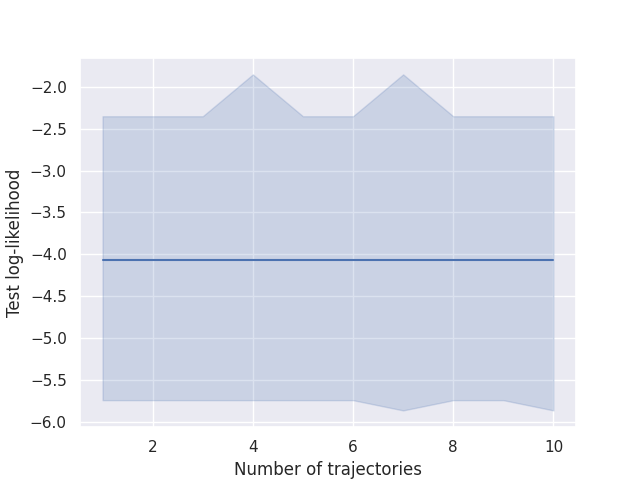
\includegraphics[width=1\linewidth]{figures/test_likelihood_particleFilter_[1.0, 0.0, 0.0]}
		\caption{}
		\label{fig:sfig2}
	\end{subfigure}
	\caption{plots of....}
	\label{fig:fig}
\end{figure}\\
$\psi_{true} =
\begin{bmatrix} \vspace{-2pt}
0.98 & 0.01 & 0.01 \\  \vspace{-2pt}
0.01 & 0.98 & 0.01 \\  \vspace{-2pt}
0.01 & 0.98 & 0.01 \\  \vspace{-1pt}
0.01 & 0.01 & 0.98
\end{bmatrix}$
$\psi_{0} =
\begin{bmatrix} \vspace{-2pt}
1 & 0 & 0 \\  \vspace{-2pt}
0 & 1 & 0 \\  \vspace{-2pt}
0 & 1 & 0 \\  \vspace{-1pt}
0 & 0 & 1
\end{bmatrix}, 
\psi_{1} =
\begin{bmatrix} \vspace{-2pt}
0 & 0 & 1 \\  \vspace{-2pt}
0 & 1 & 0 \\  \vspace{-2pt}
1 & 0 & 0 \\  \vspace{-1pt}
0 & 0 & 1 
\end{bmatrix},
\psi_{2} =
\begin{bmatrix} \vspace{-2pt}
0 & 0 & 1 \\  \vspace{-2pt}
1 & 0 & 0 \\  \vspace{-2pt}
0 & 0 & 1 \\  \vspace{-1pt}
0 & 1 & 0  
\end{bmatrix}$
\begin{figure}[htb]
	\begin{subfigure}{.5\textwidth}
		\centering
		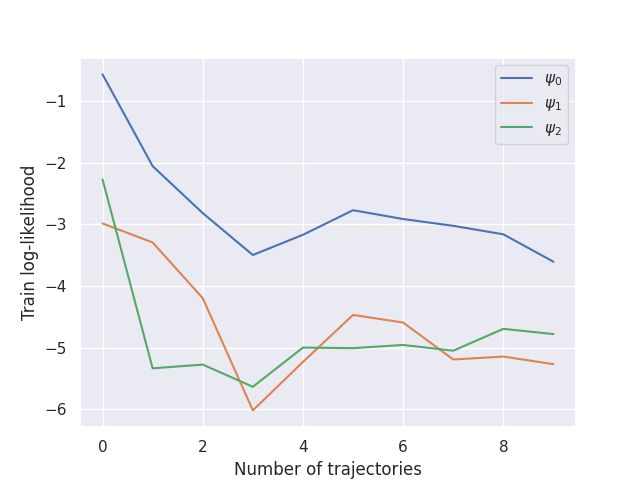
\includegraphics[width=1\linewidth]{figures/llh_[0.98, 0.01, 0.01]}
		\caption{}
		\label{fig:sfig1}
	\end{subfigure}%
	\begin{subfigure}{.5\textwidth}
		\centering
		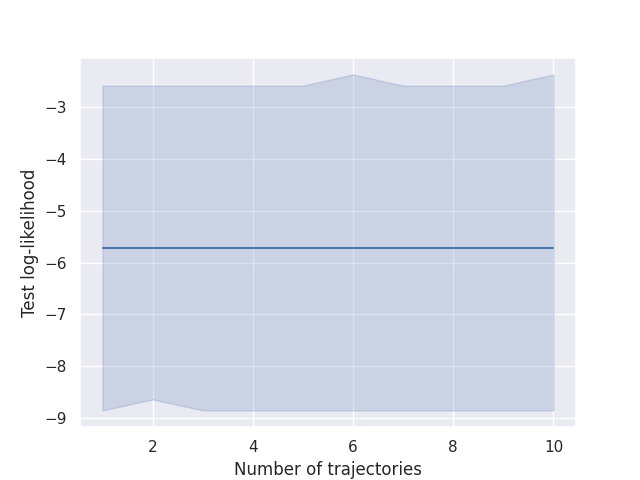
\includegraphics[width=1\linewidth]{figures/test_likelihood_particleFilter_[0.98, 0.01, 0.01]}
		\caption{}
		\label{fig:sfig2}
	\end{subfigure}
	\caption{plots of....}
	\label{fig:fig}
\end{figure}\\
$\psi_{true} =
\begin{bmatrix} \vspace{-2pt}
0.95 & 0.025 & 0.025 \\  \vspace{-2pt}
0.025 & 0.95 & 0.025 \\  \vspace{-2pt}
0.025 & 0.95 & 0.025 \\  \vspace{-1pt}
0.025 & 0.025 & 0.95
\end{bmatrix}$
$\psi_{0} =
\begin{bmatrix} \vspace{-2pt}
1 & 0 & 0 \\  \vspace{-2pt}
0 & 1 & 0 \\  \vspace{-2pt}
0 & 1 & 0 \\  \vspace{-1pt}
0 & 0 & 1
\end{bmatrix}, 
\psi_{1} =
\begin{bmatrix} \vspace{-2pt}
0 & 0 & 1 \\  \vspace{-2pt}
0 & 1 & 0 \\  \vspace{-2pt}
1 & 0 & 0 \\  \vspace{-1pt}
0 & 0 & 1 
\end{bmatrix},
\psi_{2} =
\begin{bmatrix} \vspace{-2pt}
0 & 0 & 1 \\  \vspace{-2pt}
1 & 0 & 0 \\  \vspace{-2pt}
0 & 0 & 1 \\  \vspace{-1pt}
0 & 1 & 0  
\end{bmatrix}$
\begin{figure}[htb]
	\begin{subfigure}{.5\textwidth}
		\centering
		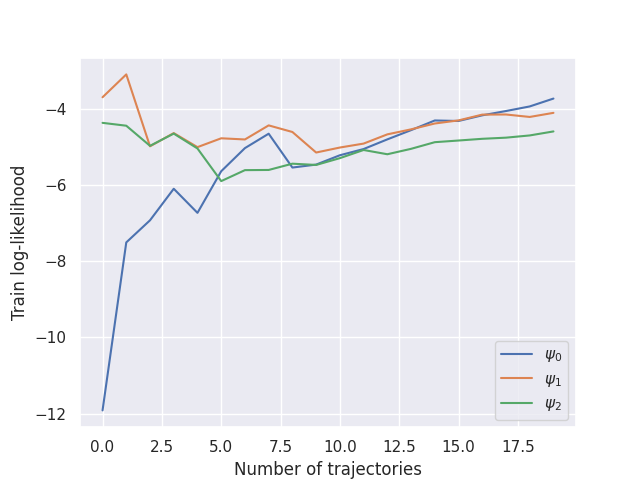
\includegraphics[width=1\linewidth]{figures/llh_particleFilter_[0.95, 0.025, 0.025]}
		\caption{}
		\label{fig:sfig1}
	\end{subfigure}%
	\begin{subfigure}{.5\textwidth}
		\centering
		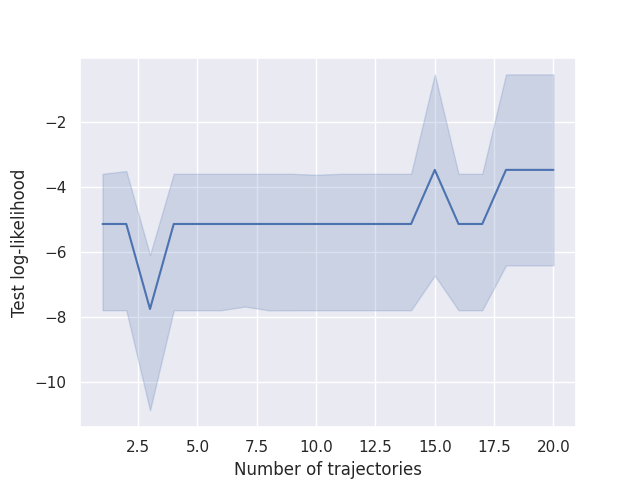
\includegraphics[width=1\linewidth]{figures/test_likelihood_particleFilter_[0.95, 0.025, 0.025]}
		\caption{}
		\label{fig:sfig2}
	\end{subfigure}
	\caption{plots of....}
	\label{fig:fig}
\end{figure}\\
$\psi_{true} =
\begin{bmatrix} \vspace{-2pt}
0.9 & 0.05 & 0.05 \\  \vspace{-2pt}
0.05 & 0.9 & 0.05 \\  \vspace{-2pt}
0.05 & 0.9 & 0.05 \\  \vspace{-1pt}
0.05 & 0.05 & 0.9
\end{bmatrix}$
$\psi_{0} =
\begin{bmatrix} \vspace{-2pt}
1 & 0 & 0 \\  \vspace{-2pt}
0 & 1 & 0 \\  \vspace{-2pt}
0 & 1 & 0 \\  \vspace{-1pt}
0 & 0 & 1
\end{bmatrix}, 
\psi_{1} =
\begin{bmatrix} \vspace{-2pt}
0 & 0 & 1 \\  \vspace{-2pt}
0 & 1 & 0 \\  \vspace{-2pt}
1 & 0 & 0 \\  \vspace{-1pt}
0 & 0 & 1 
\end{bmatrix},
\psi_{2} =
\begin{bmatrix} \vspace{-2pt}
0 & 0 & 1 \\  \vspace{-2pt}
1 & 0 & 0 \\  \vspace{-2pt}
0 & 0 & 1 \\  \vspace{-1pt}
0 & 1 & 0  
\end{bmatrix}$
\begin{figure}[htb]
	\begin{subfigure}{.5\textwidth}
		\centering
		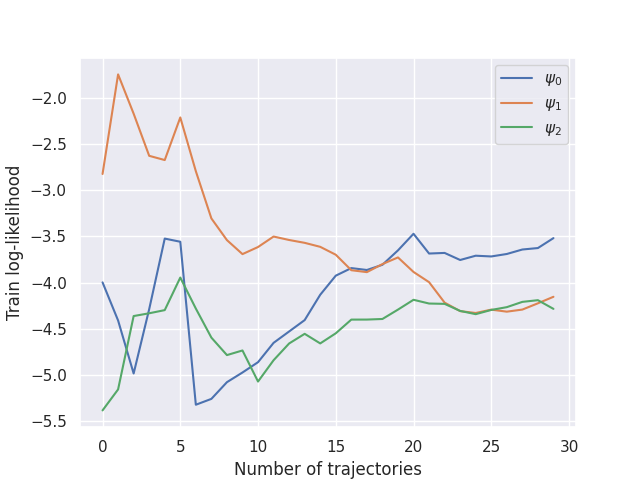
\includegraphics[width=1\linewidth]{figures/llh_particleFilter_van}
		\caption{}
		\label{fig:sfig1}
	\end{subfigure}%
	\begin{subfigure}{.5\textwidth}
		\centering
		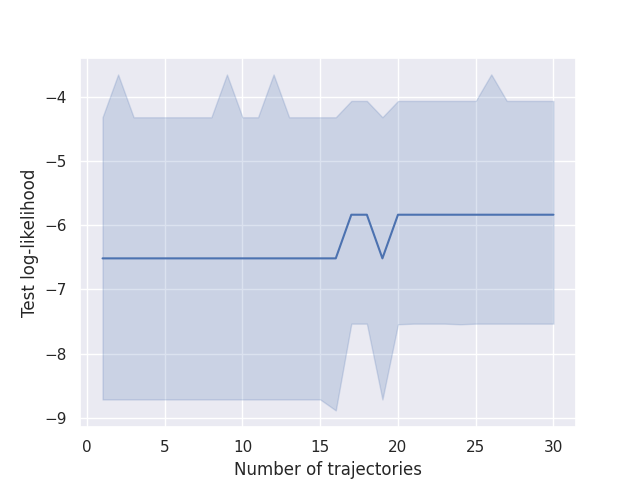
\includegraphics[width=1\linewidth]{figures/test_likelihood_particleFilter_van}
		\caption{}
		\label{fig:sfig2}
	\end{subfigure}
	\caption{plots of....}
	\label{fig:fig}
\end{figure}

\subsection{Maximum Likelihood Classification}
\begin{figure}[htb]
	\begin{subfigure}{.33\textwidth}
		\centering
		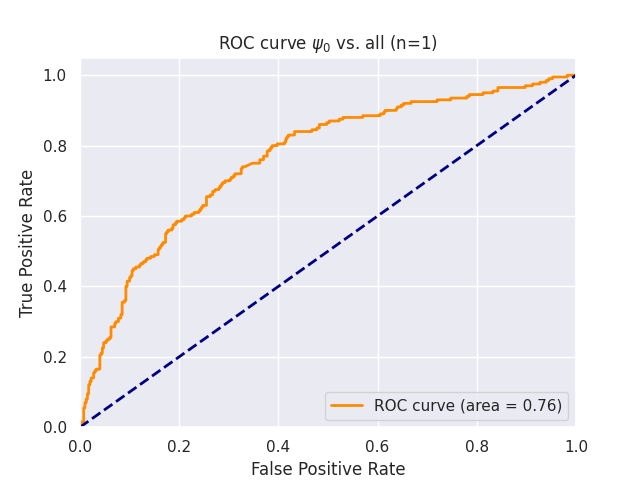
\includegraphics[width=1\linewidth]{figures/AUROC_600samples_class0_llh_n1}
		\caption{}
		\label{fig:sfig1}
	\end{subfigure}%
	\begin{subfigure}{.33\textwidth}
		\centering
		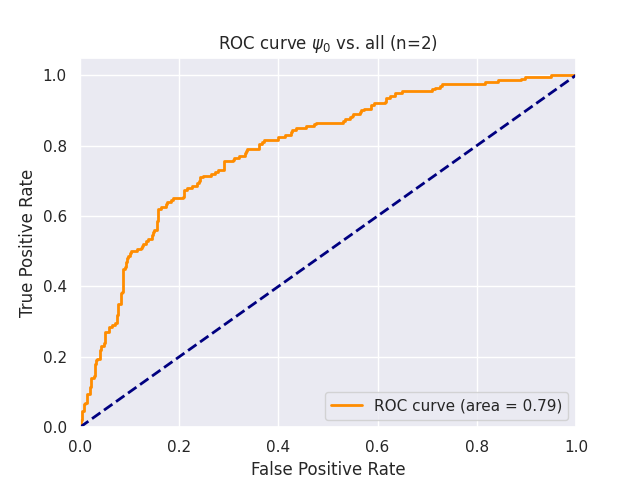
\includegraphics[width=1\linewidth]{figures/AUROC_600samples_class0_llh_n2}
		\caption{}
		\label{fig:sfig2}
	\end{subfigure}
	\begin{subfigure}{.33\textwidth}
		\centering
		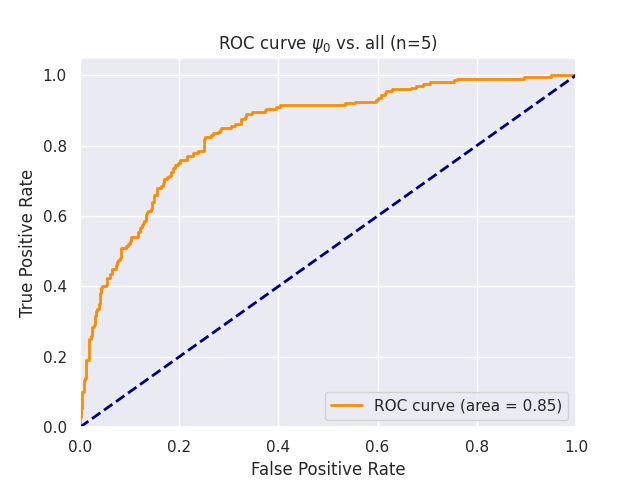
\includegraphics[width=1\linewidth]{figures/AUROC_600samples_class0_llh_n5}
		\caption{}
		\label{fig:sfig2}
	\end{subfigure}\\
	\begin{subfigure}{.33\textwidth}
		\centering
		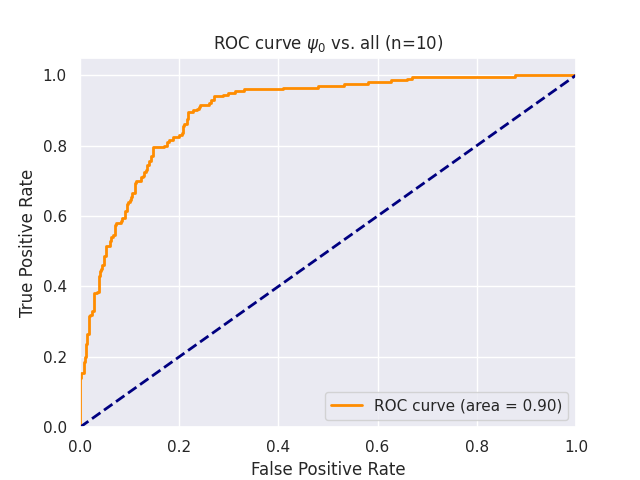
\includegraphics[width=1\linewidth]{figures/AUROC_600samples_class0_llh_n10}
		\caption{}
		\label{fig:sfig1}
	\end{subfigure}%
	\begin{subfigure}{.33\textwidth}
		\centering
		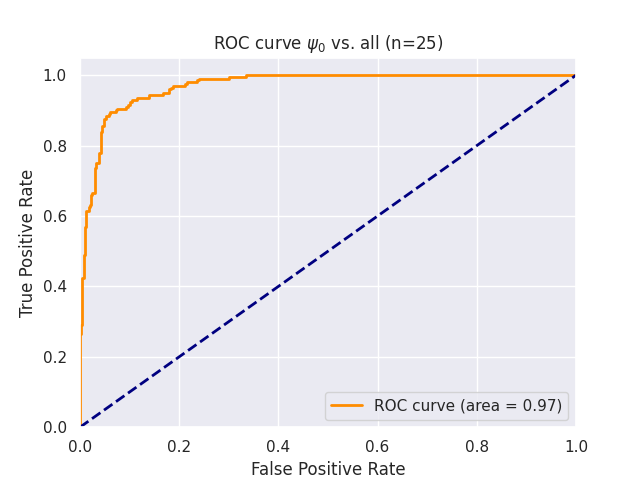
\includegraphics[width=1\linewidth]{figures/AUROC_600samples_class0_llh_n25}
		\caption{}
		\label{fig:sfig2}
	\end{subfigure}
	\begin{subfigure}{.33\textwidth}
		\centering
		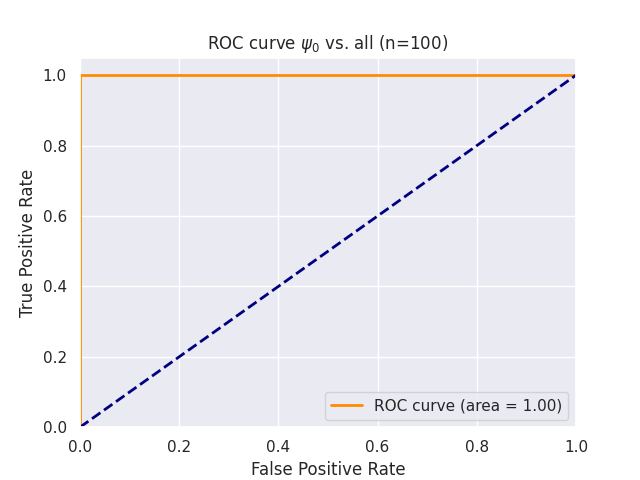
\includegraphics[width=1\linewidth]{figures/AUROC_600samples_class0_llh_n100}
		\caption{}
		\label{fig:sfig2}
	\end{subfigure}\\
	\caption{plots of....}
	\label{fig:fig}
\end{figure}
\begin{figure}[htb]
	\begin{center}
		\includegraphics[width=.9\textwidth]{figures/all_particlefilter}
		\caption{plot of...}
		\label{fig:traj}
	\end{center}
\end{figure}
